\documentclass[hyperref={pdfpagelabels=false}]{beamer}

\usepackage{focs-poster}
\usetikzlibrary{arrows.meta,positioning}

\definecolor{posterink}{HTML}{173A38}
\definecolor{posterteal}{HTML}{236B65}
\definecolor{posterblue}{HTML}{3E7198}
\definecolor{posterpurple}{HTML}{76689A}
\definecolor{postergold}{HTML}{C98B38}
\definecolor{posterpaper}{HTML}{F4F0E8}
\definecolor{postermuted}{HTML}{5F6C69}

\setbeamercolor{normal text}{fg=posterink,bg=posterpaper}
\setbeamercolor{structure}{fg=posterteal}
\setbeamercolor{itemize item}{fg=posterteal}

\newtcolorbox{musicpanel}[2][]{
  enhanced,
  colback=white,
  opacityback=.80,
  colframe=#2!55!posterink,
  opacityframe=.82,
  boxrule=.72mm,
  arc=4mm,
  left=.78cm,
  right=.78cm,
  top=.66cm,
  bottom=.66cm,
  fontupper=\fontsize{29}{35}\selectfont,
  overlay={
    \draw[#2,line width=1.35mm,line cap=round]
      ([xshift=.9cm]frame.north west) -- ([xshift=8.4cm]frame.north west);
    \draw[#2!85!posterink,line width=.72mm,line cap=round,line join=round]
      ([xshift=-8.0cm]frame.north east)
      -- ++(.75cm,0) -- ++(.30cm,.28cm) -- ++(.38cm,-.56cm)
      -- ++(.42cm,.84cm) -- ++(.46cm,-1.12cm) -- ++(.42cm,.84cm)
      -- ++(.38cm,-.56cm) -- ++(.30cm,.28cm) -- ++(.75cm,0);
    \begin{scope}
      \clip (interior.south west) rectangle (interior.north east);
      \coordinate (groove) at ([xshift=-.15cm,yshift=.15cm]interior.south east);
      \draw[#2,opacity=.12,line width=.65mm] (groove) circle (1.55cm);
      \draw[#2,opacity=.12,line width=.65mm] (groove) circle (2.45cm);
      \draw[#2,opacity=.12,line width=.65mm] (groove) circle (3.35cm);
      \fill[#2,opacity=.15] (groove) circle (.28cm);
    \end{scope}
  },
  #1
}

\newcommand{\sectiontitle}[1]{%
  {\fontsize{44}{49}\selectfont\bfseries\color{posterink}#1\par}%
}

\newcommand{\smallnote}[1]{%
  {\fontsize{25}{30}\selectfont\color{postermuted}#1\par}%
}

\newcommand{\yearbar}[4]{%
  \node[anchor=east,font=\bfseries] at (0,#1+.34) {#2};
  \fill[#4,rounded corners=.8mm] (.35,#1) rectangle ({.35+#3*.78},#1+.68);
  \node[anchor=west,font=\bfseries] at ({.58+#3*.78},#1+.34) {#3};
}

\usebackgroundtemplate{%
  \begin{tikzpicture}[remember picture,overlay]
    \node[inner sep=0] at (current page.center) {%
      \includegraphics[height=\paperheight]{img/music-intelligence-background.png}%
    };
  \end{tikzpicture}%
}

\begin{document}

\begin{frame}

% Title artwork ---------------------------------------------------------------
\begin{textblock}{92}(4,1.7)
  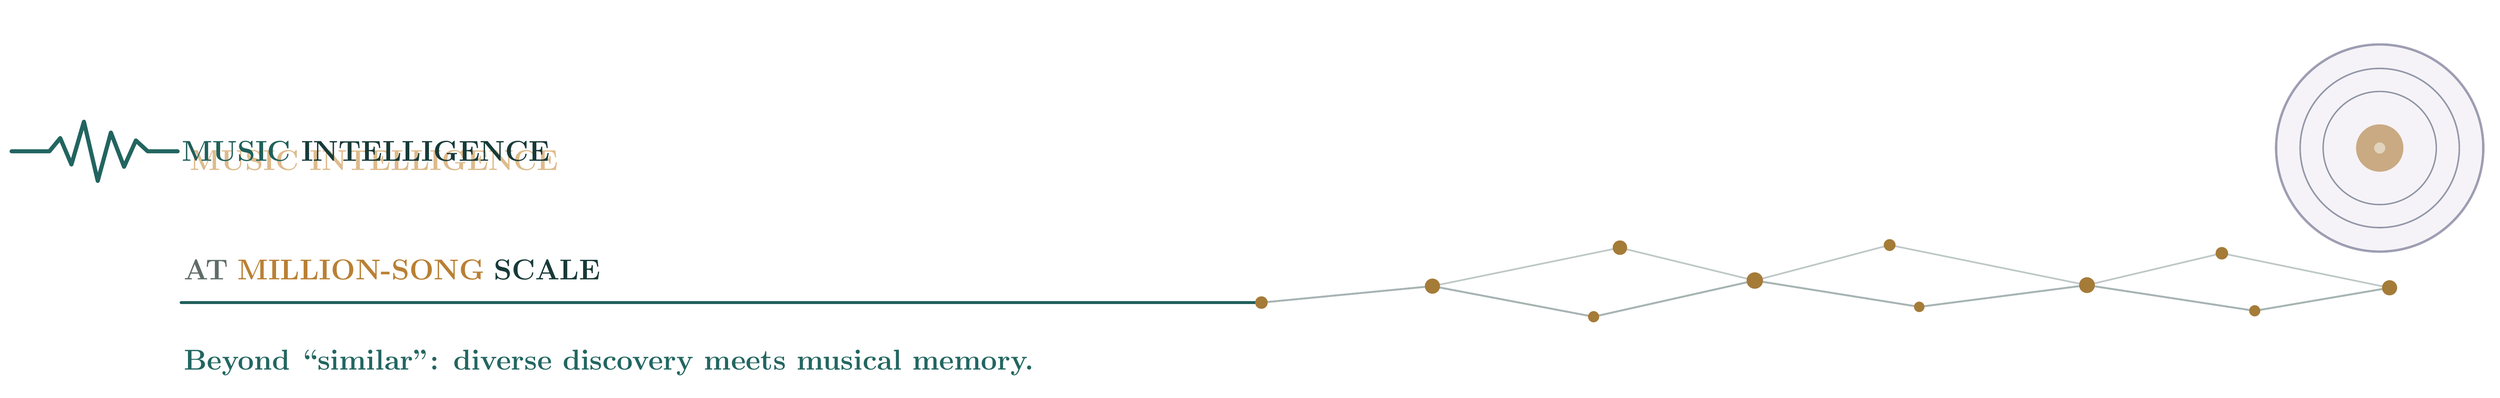
\begin{tikzpicture}[x=1cm,y=1cm,baseline=(current bounding box.north)]
    \path[use as bounding box] (0,0) rectangle (75.3,11.4);

    % A music waveform enters the wordmark from the left.
    \draw[posterteal!88!posterink,line width=1.25mm,line cap=round,line join=round]
      (0,7.15) -- (1.15,7.15) -- (1.48,7.55) -- (1.82,6.75)
      -- (2.20,8.05) -- (2.62,6.25) -- (3.02,7.72)
      -- (3.42,6.68) -- (3.78,7.48) -- (4.14,7.15) -- (5.05,7.15);

    % Warm offset print shadow, followed by the crisp foreground lettering.
    \node[anchor=west,font=\fontsize{104}{108}\selectfont\bfseries,
      text=postergold!52!posterpaper] at (5.30,6.88)
      {MUSIC INTELLIGENCE};
    \node[anchor=west,font=\fontsize{104}{108}\selectfont\bfseries]
      at (5.05,7.15)
      {{\color{posterteal!78!posterink}MUSIC}\hspace{.32cm}{\color{posterink}INTELLIGENCE}};

    \node[anchor=west,font=\fontsize{45}{50}\selectfont\bfseries]
      at (5.12,3.55)
      {{\color{postermuted}AT}\hspace{.28cm}{\color{postergold!92!black}MILLION-SONG}\hspace{.28cm}{\color{posterink}SCALE}};

    % The signal becomes a small data network under the scale line.
    \draw[posterteal!76!posterink,line width=.78mm,line cap=round]
      (5.15,2.55) -- (38.0,2.55);
    \draw[posterink!38,line width=.58mm]
      (38.0,2.55) -- (43.2,3.05) -- (48.1,2.12) -- (53.0,3.22)
      -- (58.0,2.42) -- (63.1,3.08) -- (68.2,2.30) -- (72.3,3.00);
    \draw[posterink!28,line width=.50mm]
      (43.2,3.05) -- (48.9,4.22) -- (53.0,3.22) -- (57.1,4.30)
      -- (63.1,3.08) -- (67.2,4.05) -- (72.3,3.00);
    \foreach \x/\y/\r in {
      38.0/2.55/.19,43.2/3.05/.23,48.1/2.12/.17,48.9/4.22/.22,
      53.0/3.22/.25,57.1/4.30/.18,58.0/2.42/.16,63.1/3.08/.24,
      67.2/4.05/.19,68.2/2.30/.17,72.3/3.00/.23}
      \fill[postergold!80!posterink] (\x,\y) circle (\r cm);

    % A subtle record anchors the nostalgic side of the identity.
    \begin{scope}[opacity=.58]
      \fill[posterpurple!13] (72.0,7.25) circle (3.15cm);
      \draw[posterpurple!72!posterink,line width=.72mm] (72.0,7.25) circle (3.15cm);
      \draw[posterpurple!58!posterink,line width=.46mm] (72.0,7.25) circle (2.42cm);
      \draw[posterpurple!48!posterink,line width=.42mm] (72.0,7.25) circle (1.72cm);
      \fill[postergold!85!black] (72.0,7.25) circle (.72cm);
      \fill[posterpaper] (72.0,7.25) circle (.17cm);
    \end{scope}

    \node[anchor=west,font=\fontsize{31}{37}\selectfont\bfseries,
      text=posterteal!90!posterink] at (5.12,.72)
      {Beyond ``similar'': diverse discovery meets musical memory.};
  \end{tikzpicture}
\end{textblock}

% Product story ----------------------------------------------------------------
% Disabled while the title artwork is being designed.
\newcommand{\disabledtargetpanel}{%
\begin{textblock}{58}(4,13.0)
  \begin{musicpanel}[height=16.2cm]{posterteal}
    \sectiontitle{Our target: one song, three experiences.}
    \vspace{.12cm}
    {\fontsize{28}{34}\selectfont\color{postermuted}
      Turn one query into catalog insight, diverse recommendations, and a journey through musical time.\par}
    \vspace{.08cm}
    \begin{center}
      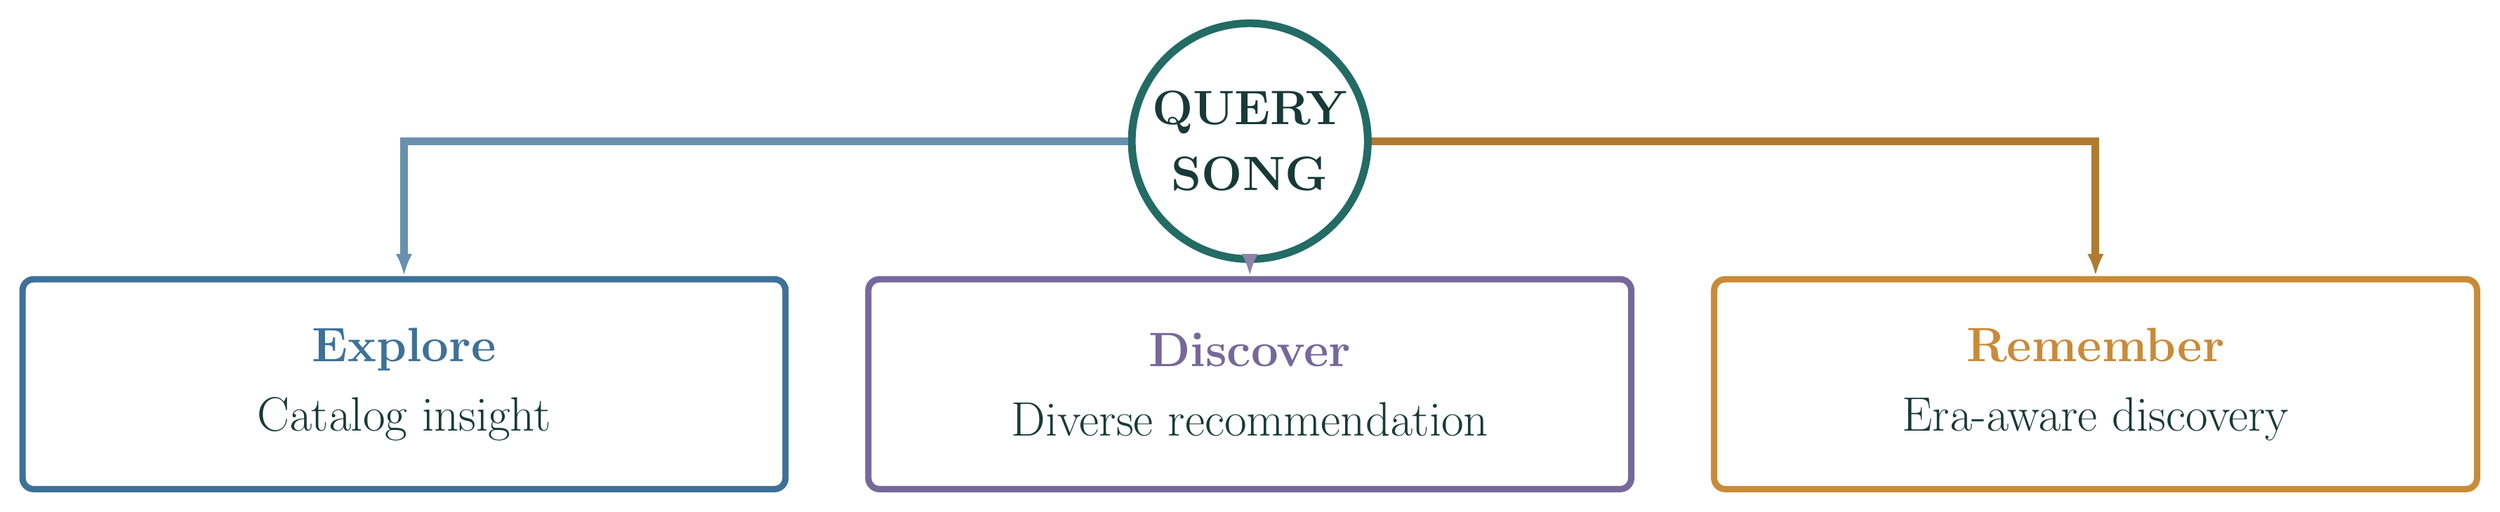
\begin{tikzpicture}[
        >=Latex,
        flow/.style={-{Latex[length=4mm,width=3mm]},line width=1.4mm},
        query/.style={circle,minimum size=3.65cm,line width=1.4mm,
          draw=posterteal,fill=white,fill opacity=.72,text opacity=1,
          font=\fontsize{30}{34}\selectfont\bfseries,align=center,text=posterink},
        outcome/.style={rounded corners=2mm,minimum width=13.8cm,minimum height=3.8cm,
          line width=1.15mm,align=center,fill=white,fill opacity=.68,text opacity=1,
          font=\fontsize{28}{33}\selectfont,text=posterink}
      ]
        \node[query] (song) at (0,2.35) {QUERY\\SONG};

        \node[outcome,draw=posterblue] (explore) at (-15.3,-2.05) {
          {\fontsize{34}{38}\selectfont\bfseries\color{posterblue}Explore}\\[.10cm]
          Catalog insight};
        \node[outcome,draw=posterpurple] (discover) at (0,-2.05) {
          {\fontsize{34}{38}\selectfont\bfseries\color{posterpurple}Discover}\\[.10cm]
          Diverse recommendation};
        \node[outcome,draw=postergold] (remember) at (15.3,-2.05) {
          {\fontsize{34}{38}\selectfont\bfseries\color{postergold}Remember}\\[.10cm]
          Era-aware discovery};

        \draw[flow,draw=posterblue!78] (song.west) -| (explore.north);
        \draw[flow,draw=posterpurple!82] (song.south) -- (discover.north);
        \draw[flow,draw=postergold!88!black] (song.east) -| (remember.north);
      \end{tikzpicture}
    \end{center}
    \vspace{-.20cm}
    \begin{center}
      {\fontsize{27}{32}\selectfont\bfseries\color{posterink}
        Big-data method: 267 GB HDF5 $\rightarrow$ Avro/Parquet $\rightarrow$ Drill + Spark $\rightarrow$ FAISS + learned models}
    \end{center}
  \end{musicpanel}
\end{textblock}
}

% Better discovery -------------------------------------------------------------
\begin{textblock}{29.5}(4,59.2)
  \begin{musicpanel}[height=19.0cm]{posterpurple}
    \sectiontitle{Better discovery}
    \smallnote{Relation-aware vs. release-only retrieval}
    \vspace{.65cm}

    \begin{center}
      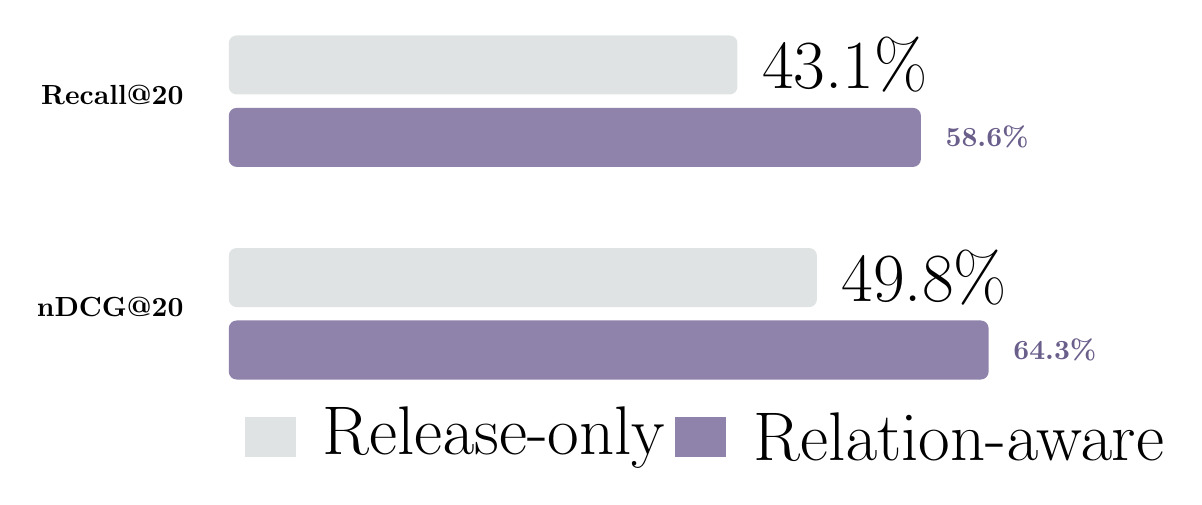
\begin{tikzpicture}[x=1cm,y=1cm,font=\fontsize{23}{27}\selectfont]
        \node[anchor=east,font=\bfseries] at (0,3.60) {Recall@20};
        \node[anchor=east,font=\bfseries] at (0,.90) {nDCG@20};

        \fill[posterink!14,rounded corners=1mm] (.45,3.60) rectangle (6.91,4.35);
        \fill[posterpurple!82,rounded corners=1mm] (.45,2.68) rectangle (9.24,3.43);
        \fill[posterink!14,rounded corners=1mm] (.45,.90) rectangle (7.92,1.65);
        \fill[posterpurple!82,rounded corners=1mm] (.45,-.02) rectangle (10.10,.73);

        \node[anchor=west] at (7.10,3.98) {43.1\%};
        \node[anchor=west,font=\bfseries,text=posterpurple!90!black] at (9.43,3.06) {58.6\%};
        \node[anchor=west] at (8.11,1.28) {49.8\%};
        \node[anchor=west,font=\bfseries,text=posterpurple!90!black] at (10.29,.36) {64.3\%};

        \fill[posterink!14] (.65,-1.00) rectangle (1.30,-.50);
        \node[anchor=west] at (1.52,-.75) {Release-only};
        \fill[posterpurple!82] (6.12,-1.00) rectangle (6.77,-.50);
        \node[anchor=west] at (6.99,-.75) {Relation-aware};
      \end{tikzpicture}
    \end{center}

    \vspace{.65cm}
    \begin{center}
      {\fontsize{58}{62}\selectfont\bfseries\color{posterpurple}+15.6 pp\par}
      {\fontsize{31}{36}\selectfont\bfseries Recall@20\par}
      \vspace{.35cm}
      {\fontsize{31}{36}\selectfont\bfseries\color{posterink}+14.5 pp nDCG@20\par}
    \end{center}

    \vfill
    \begin{center}
      {\fontsize{25}{30}\selectfont\color{postermuted}10,000-query offline benchmark}
    \end{center}
  \end{musicpanel}
\end{textblock}

% Faster graph intelligence ----------------------------------------------------
\begin{textblock}{29.5}(35.25,42.8)
  \begin{musicpanel}[height=19.0cm]{posterblue}
    \sectiontitle{Faster graph intelligence}
    \smallnote{Same graph. Same verified answer.}
    \vspace{.65cm}

    \begin{center}
      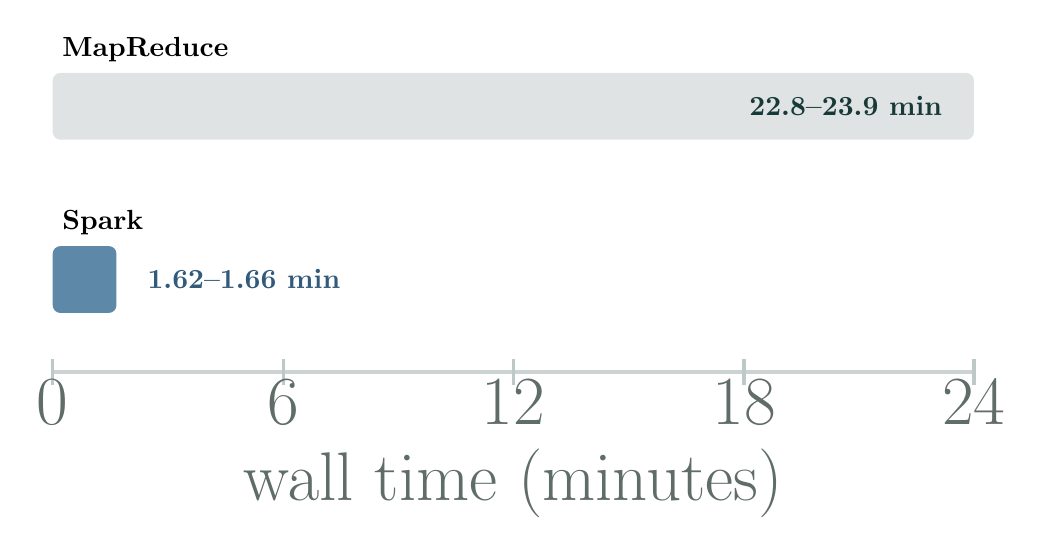
\begin{tikzpicture}[x=1cm,y=1cm,font=\fontsize{24}{28}\selectfont]
        \node[anchor=west,font=\bfseries] at (0,4.45) {MapReduce};
        \fill[posterink!14,rounded corners=1mm] (0,3.30) rectangle (11.7,4.15);
        \node[anchor=east,font=\bfseries,text=posterink] at (11.42,3.73) {22.8--23.9 min};

        \node[anchor=west,font=\bfseries] at (0,2.25) {Spark};
        \fill[posterblue!84,rounded corners=1mm] (0,1.10) rectangle (.81,1.95);
        \node[anchor=west,font=\bfseries,text=posterblue!80!black] at (1.08,1.53) {1.62--1.66 min};

        \draw[line width=.55mm,draw=posterink!22] (0,.35) -- (11.7,.35);
        \foreach \x/\lab in {0/0,2.93/6,5.85/12,8.78/18,11.7/24}
          \draw[draw=posterink!28,line width=.4mm] (\x,.18) -- (\x,.52)
            node[below=.14cm,text=postermuted] {\lab};
        \node[below=.85cm,text=postermuted] at (5.85,.35) {wall time (minutes)};
      \end{tikzpicture}
    \end{center}

    \vspace{.70cm}
    \begin{center}
      {\fontsize{58}{62}\selectfont\bfseries\color{posterblue}14.1--14.4$\times$\par}
      {\fontsize{31}{36}\selectfont\bfseries faster with Spark\par}
    \end{center}

    \vfill
    \begin{center}
      {\fontsize{25}{30}\selectfont\color{postermuted}Five runs per combination . all outputs verified}
    \end{center}
  \end{musicpanel}
\end{textblock}

% Sharper era estimation -------------------------------------------------------
\begin{textblock}{29.5}(66.5,26.4)
  \begin{musicpanel}[height=19.0cm]{postergold}
    \sectiontitle{Sharper era estimation}
    \smallnote{Progressive improvement on held-out artists}
    \vspace{.55cm}

    \begin{center}
      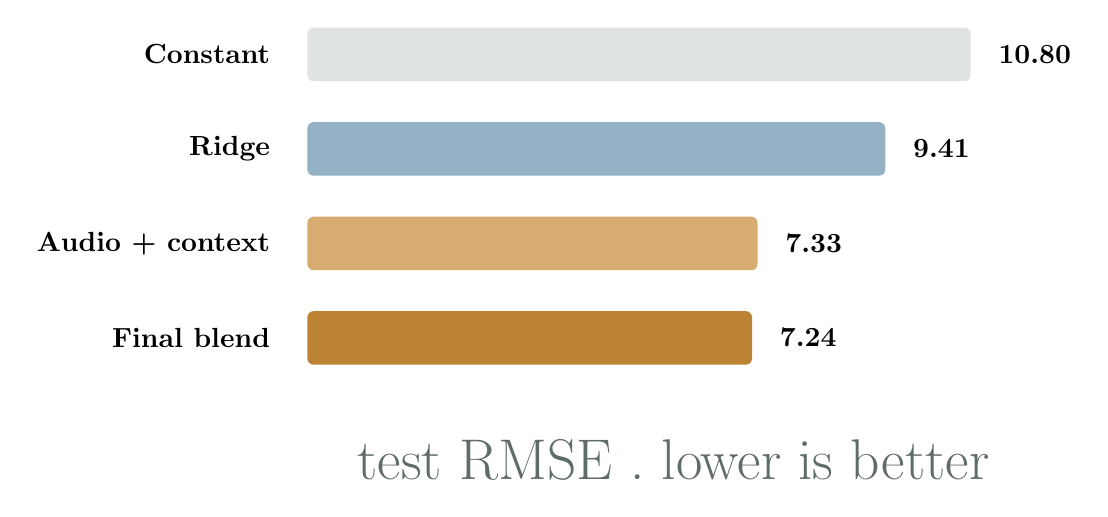
\begin{tikzpicture}[x=1cm,y=1cm,font=\fontsize{21}{25}\selectfont]
        \yearbar{3.65}{Constant}{10.80}{posterink!14}
        \yearbar{2.45}{Ridge}{9.41}{posterblue!55}
        \yearbar{1.25}{Audio + context}{7.33}{postergold!72}
        \yearbar{.05}{Final blend}{7.24}{postergold!94!black}
        \node[anchor=north,text=postermuted] at (5.0,-.78) {test RMSE . lower is better};
      \end{tikzpicture}
    \end{center}

    \vspace{.60cm}
    \begin{center}
      {\fontsize{58}{62}\selectfont\bfseries\color{postergold}7.24 years\par}
      {\fontsize{31}{36}\selectfont\bfseries final test RMSE\par}
      \vspace{.35cm}
      {\fontsize{31}{36}\selectfont\bfseries\color{posterink}23.0\% lower than Ridge\par}
      \vspace{.28cm}
      {\fontsize{27}{32}\selectfont\color{postermuted}Final MAE: 4.82 years\par}
    \end{center}

  \end{musicpanel}
\end{textblock}

% Investment close -------------------------------------------------------------
% Disabled while the title artwork is being designed.
\newcommand{\disabledinvestmentpanel}{%
\begin{textblock}{38}(58,76.6)
  \begin{musicpanel}[height=9.6cm]{posterteal}
    \sectiontitle{Why invest now?}
    \vspace{.52cm}
    {\fontsize{31}{36}\selectfont\bfseries\color{posterpurple}Differentiated}\quad
    {\fontsize{27}{32}\selectfont Discovery beyond nearest-neighbor lists.\par}
    \vspace{.42cm}
    {\fontsize{31}{36}\selectfont\bfseries\color{posterblue}Measured}\quad
    {\fontsize{27}{32}\selectfont One million tracks, reproducible evidence.\par}
    \vspace{.42cm}
    {\fontsize{31}{36}\selectfont\bfseries\color{postergold}Ready to learn}\quad
    {\fontsize{27}{32}\selectfont Online listener feedback is next.\par}
  \end{musicpanel}
\end{textblock}
}

% Footer ----------------------------------------------------------------------
\begin{textblock}{92}(4,95.4)
  {\fontsize{25}{30}\selectfont\bfseries\color{posterink}
    Jiang Ruiyu . Li Zhiyuan . Yao Yunxiang . Zhang Jingkai}
\end{textblock}

\end{frame}

\end{document}
